\documentclass[11pt,a4paper]{article}

% ---------- Packages ----------
\usepackage[utf8]{inputenc}
\usepackage[T1]{fontenc}
\usepackage{lmodern}
\usepackage{graphicx}
\usepackage{amsmath, amssymb}
\usepackage{booktabs}
\usepackage{hyperref}
\usepackage[margin=1in]{geometry}
\usepackage{caption}
\usepackage{subcaption}
\usepackage{enumitem}
\usepackage{float}     % for [H] exact figure placement
\usepackage{placeins}  % for \FloatBarrier

\hypersetup{
    colorlinks=true,
    linkcolor=blue,
    citecolor=blue,
    urlcolor=blue
}

% Where figures live
\graphicspath{{figs/}}

\title{\textbf{Horse$\leftrightarrow$Zebra Image Translation Using CycleGAN}}
\author{Md Naim Hassan Saykat}
\date{}

\begin{document}
\maketitle

\begin{abstract}
This project implements Cycle-Consistent Adversarial Networks (CycleGAN) in PyTorch for unpaired image-to-image translation between horses and zebras. The notebook shows qualitative results, configures training with adversarial and cycle-consistency losses, and specifies generator and discriminator architectures. The Structural Similarity Index (SSIM) and Peak Signal-to-Noise Ratio (PSNR) are used to assess the outputs of learning both horse-to-zebra and zebra-to-horse mappings.
\end{abstract}

\noindent \textbf{Keywords:} CycleGAN, unpaired image translation, GANs, horse2zebra, computer vision.

\section{Introduction}
Image-to-image translation learns mappings between visual domains. Unlike supervised approaches such as pix2pix \cite{Isola2017Pix2Pix}, CycleGAN \cite{Zhu2017CycleGAN} enables training without paired samples by enforcing cycle-consistency. In this project, we apply CycleGAN to the horse2zebra dataset to demonstrate unpaired domain translation.

\section{Methodology}
\textbf{Generator:} U-Net-like encoder--decoder with residual blocks. \\
\textbf{Discriminator:} PatchGAN classifier that distinguishes real vs.\ fake local patches. \\
\textbf{Losses:}
\begin{itemize}[leftmargin=1.25em]
    \item Adversarial loss (MSE)
    \item Cycle-consistency loss (L1)
\end{itemize}
\textbf{Optimization:} Adam optimizer with learning rate $2 \times 10^{-4}$, $\beta_1=0.5$, $\beta_2=0.999$.

\section{Dataset}
The project uses the horse2zebra dataset provided by the CycleGAN authors \cite{Zhu2017CycleGAN}. It consists of unpaired training images from both domains. Images are resized to $256 \times 256$, normalized to $[-1, 1]$, and randomly shuffled for training.

\section{Experiments}
\begin{itemize}[leftmargin=1.25em]
    \item \textbf{Training:} 100 epochs, batch size 1.
    \item \textbf{Checkpoints:} Generators saved every 10 epochs.
    \item \textbf{Inference:} After training, the models are set to evaluation mode for generation.
\end{itemize}

\subsection{Qualitative Results: Horse$\rightarrow$Zebra}
Figure~\ref{fig:h2z} shows a grid of real horses and their translated zebras produced by the trained model.
\begin{figure}[H]
    \centering
    \begin{subfigure}{0.48\textwidth}
        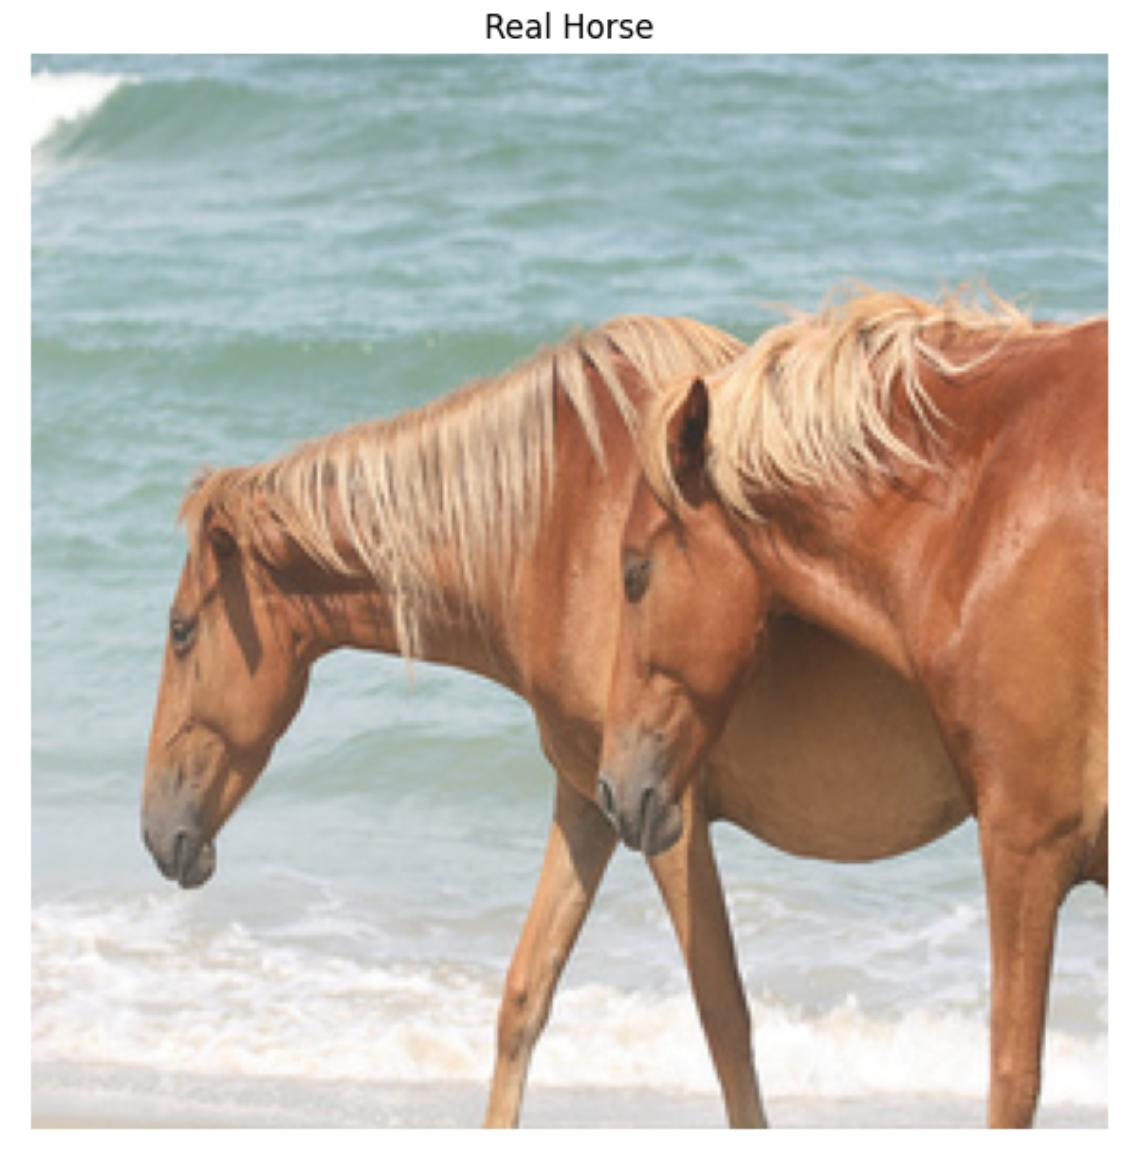
\includegraphics[width=\linewidth]{real_horses.png}
        \caption{Real Horses}
    \end{subfigure}\hfill
    \begin{subfigure}{0.48\textwidth}
        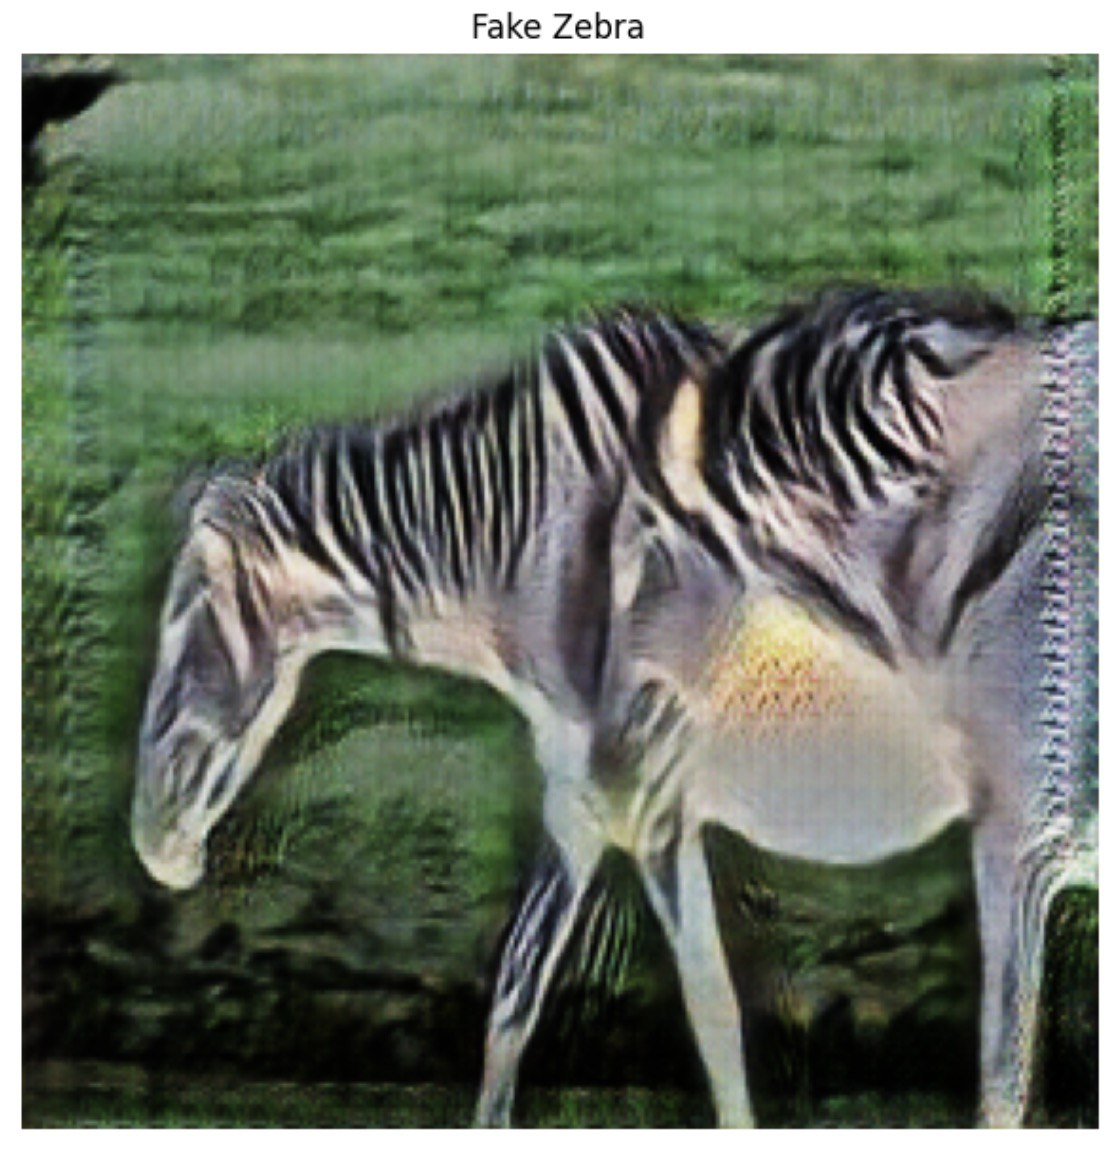
\includegraphics[width=\linewidth]{fake_zebras.png}
        \caption{Generated Zebras}
    \end{subfigure}
    \caption{Qualitative example of horse$\rightarrow$zebra translation using CycleGAN.}
    \label{fig:h2z}
\end{figure}

\subsection{Qualitative Results: Zebra$\rightarrow$Horse}
Figure~\ref{fig:z2h} presents real zebras and their translated horses.
\begin{figure}[H]
    \centering
    \begin{subfigure}{0.48\textwidth}
        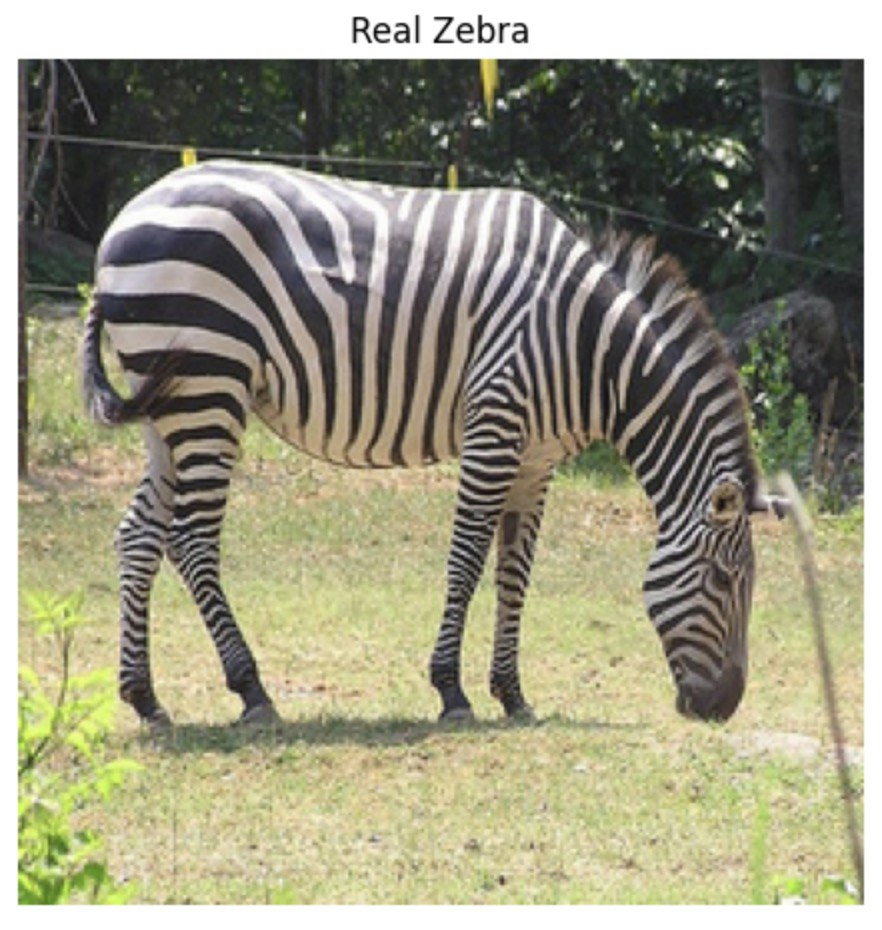
\includegraphics[width=\linewidth]{real_zebras.png}
        \caption{Real Zebras}
    \end{subfigure}\hfill
    \begin{subfigure}{0.48\textwidth}
        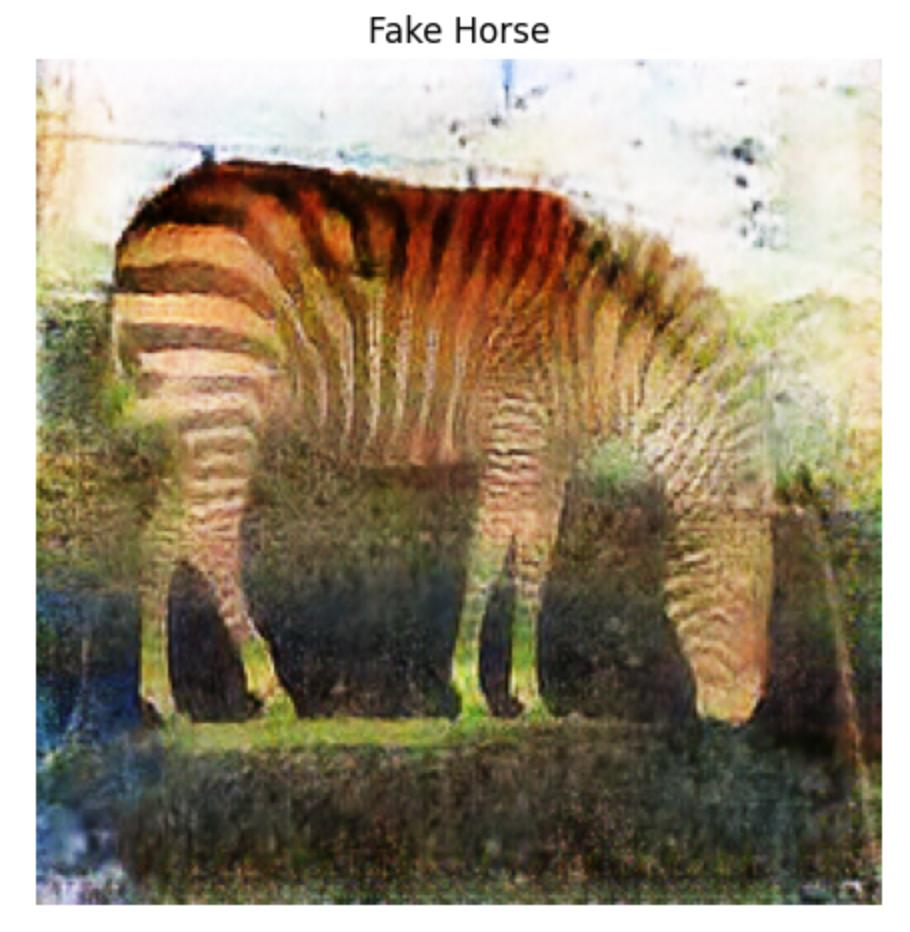
\includegraphics[width=\linewidth]{fake_horses.png}
        \caption{Generated Horses}
    \end{subfigure}
    \caption{Qualitative example of zebra$\rightarrow$horse translation using CycleGAN.}
    \label{fig:z2h}
\end{figure}

\FloatBarrier

\subsection{Quantitative Results}
Average SSIM and PSNR were computed over 10 samples to provide an objective comparison of real vs.\ translated images. These pixel-level metrics offer a basic sanity check but are known to be limited for unpaired translation \cite{Wang2004SSIM}.

\section{Results and Discussion}
In both directions, the CycleGAN model exhibits believable style transfer. Although qualitative results demonstrate compelling stripe transfer, there are sporadic structural distortions and background artifacts. SSIM and PSNR scores confirm moderate similarity, consistent with known limitations of pixel-based evaluation in unpaired translation tasks.

\section{Limitations and Future Work}
\begin{itemize}[leftmargin=1.25em]
    \item Background regions are sometimes incorrectly stylized.
    \item Fine details (e.g., legs, tails) can appear distorted.
    \item Future extensions may include perceptual metrics such as FID \cite{Heusel2017FID}, LPIPS \cite{Zhang2018LPIPS}, and attention-based generators.
\end{itemize}

\section{Conclusion}
A working PyTorch implementation of CycleGAN for horse-zebra translation is presented in this notebook.  Adversarial and cycle-consistency losses are used to learn both directions, and straightforward quantitative indicators and qualitative visualization are used to validate the findings.  The research highlights opportunities for improvement while showcasing the efficacy of unpaired picture translation.

\bibliographystyle{plain}
\bibliography{references}

\end{document}